\documentclass[12pt]{article}

\usepackage{preamble}
\usepackage{xgames}
\usepackage{fikz}
\addbibresource{references.bib}

\graphicspath{{../figures/}}
%%%%%%%%%%%%%%%%%%%%%%%%%%%%%%%%%%%%%%%%%%%%%%%%%%%%%%%%%%%

%\usepackage{amsfonts, amsmath}
\usepackage{amssymb, geometry}
\usepackage{commath}
\usepackage{comment}
\usepackage{scalefnt}
\usepackage{setspace}
\usepackage{color,hyperref}
%\usepackage{epsfig,subfigure,morefloats}
\usepackage{dsfont}
\usepackage{epstopdf}
%\usepackage{amsthm}
\usepackage{graphicx}
\usepackage{booktabs,siunitx}
\usepackage{bm}
\usepackage[section]{placeins}
%\usepackage{hypcap}
\usepackage{afterpage}
\usepackage[makeroom]{cancel}


%%%%%%%%%%%%%%%%%%%%%%%%%%%%%%%%%%%%%%%%%%%%%%%%%%%%%%%%%%%

\geometry{left=1in,right=1in,top=1in,bottom=1in}

%%%%%%%%%%%%%%%%%%%%%%%%%%%%%%%%%%%%%%%%%%%%%%%%%%%%%%%%%%%
\usepackage{float}
\usepackage{indentfirst}
\usepackage{listings}
\usepackage{subcaption} 
\usepackage[toc,page]{appendix}
\usepackage{tocloft}
\usepackage{mathtools}


\usepackage{mathpazo} % math & rm
\linespread{1.15}        % Palatino needs more leading (space between lines)
\usepackage[scaled]{helvet} % ss
\usepackage{courier} % tt
\normalfont
\usepackage[T1]{fontenc}
\setcounter{tocdepth}{4}
\newcommand{\R}{\mathbb{R}}
\newcommand{\C}{\mathbb{C}}
\newcommand{\Z}{\mathbb{Z}}
\newcommand{\N}{\mathbb{N}}
\newcommand{\Q}{\mathbb{Q}}
\newcommand{\E}{\mathbb{E}}
\newcommand{\p}{\mathbb{P}}
\newcommand{\G}{\mathcal{G}}
\newcommand{\I}{\mathcal{I}}
\newcommand{\A}{\mathcal{A}}
\newcommand{\M}{\mathcal{M}}
\newcommand{\B}{\mathcal{B}}
\newcommand{\F}{\mathcal{F}}
\newcommand{\J}{\mathcal{J}}
% \newcommand{\Pr}{\mathbb{P}}
\newcommand{\thetahat}{\hat{\theta}}
\newcommand{\Qhat}{\hat{\mathbb{Q}}}
\newcommand{\logn}{\ell n}
\newcommand{\iid}{\stackrel{\mathclap{iid}}{\sim}}
\newcommand{\notimplies}{%
\mathrel{{\ooalign{\hidewidth$\not\phantom{=}$\hidewidth\cr$\implies$}}}}
\newcommand{\WTS}{\colorbox{lightblue!20}{\textbf{WTS.}} }
\newcommand{\Cov}{\mathrm{Cov}}
\newcommand{\Var}{\mathrm{Var}}


%\usepackage{bookman}
%\usepackage{palatino}
\usepackage{lmodern}
%\usepackage{pifont}
% \usepackage{pxfonts}
%\usepackage{tgpagella}
%\usepackage{utfsym}


\newcommand{\cmark}{\ding{51}}%
\newcommand{\xmark}{\ding{55}}%
\newcommand{\crossmark}{\usym{2717}}

\newcommand*\circled[1]{\tikz[baseline=(char.base)]{
            \node[shape=circle,draw,inner sep=0.5pt] (char) {#1};}}

\usepackage[bottom]{footmisc} % Ensures footnotes appear at the bottom of the page

\numberwithin{equation}{section}
%%%%%%%%%%%%%%%%%%%%%%%%%%%%%%%%%%%%%%%%%%%%%%%%%%%%%%%%%%%
\title{\huge Fall25 ECON880 PSET2}
\author{\Large Eric Hsienchen Chu\footnote{Department of Finance, Wisconsin School of Business. 
\href{mailto:hchu38@wisc.edu}{hchu38@wisc.edu}. 
This is PSET for ECON 880: Computational Methods in Fall 2025. 
Instructors: Prof. Dean Corbae and Prof. Rasmus Lentz.}}

\begin{document}
\date{\Large Due: September 19, 2025}
\maketitle
\renewcommand{\cftdot}{.}

%\listoftodos[Appendix]
%\improvement[inline]{Todo.}

%\tableofcontents
\vspace{-4ex}
%\newpage

% ------ Section 1 ------%
\section{Huggett (1993, JEDC)}
%%%%%%%%%%%%% Q1 %%%%%%%%%%%%%
\begin{framedexercise}[Competitive EQM] Consider the same environment as \citet{Huggett1993-sn} except assume
    that there are enforceable insurance markets regarding the idiosyncratic shocks
    to earnings and that there are no initial asset holdings. Solve for a competitive
    equilibrium. What are prices? What is the allocation? (Hint: think about the
    planner’s problem and then decentralize)
\end{framedexercise}

\begin{solution} (I follow the notations in slides.) The environment is as follows:
    \begin{itemize}
        \item Population: unit measure of HH.
        \item Preferences: $\E_0 \left[ \displaystyle\sum_{t=0}^{\infty} \beta^t U(c_t)\right]$,
              where $U$ is continuously differentiable, strictly concave, and bounded.
        \item Endowment: $s_t \in \mathcal{S} = \{e, u\}$ (earning shocks, which are i.i.d. across HH)
              \begin{itemize}
                  \item Earns $y^e = 1$ if employed; earns $y^u = 0.5$ if unemployed
                  \item Markov employment process: $\mathcal{P} = \begin{bmatrix}
                                \pi(e|e) & \pi(u|e) \\
                                \pi(e|u) & \pi(u|u)
                            \end{bmatrix} = \begin{bmatrix}
                                {0.97} & 0.03  \\
                                0.5    & {0.5}
                            \end{bmatrix}$.\footnote{Use
                            duration of unemployment data of 2 quarters and an average unemployment rate
                            of 6$\%$}
                  \item We can invariant dist by $\Pi \mathcal{P} = \Pi \implies \Pi = \left\{\pi_e, \pi_u\right\} = \left\{0.94, 0.06\right\}$
              \end{itemize}
        \item Asset: non-contingent bonds $a_t \in A$ with price of next-period bonds $q_t$ (for $a_{t+1}$); borrowing constraint $\underline{a} \leq 0$
        \item Other: discount factor $\beta = 0.9932$; relative risk aversion $\alpha = 1.5$
    \end{itemize} \textit{(Cont'd on next page!)}
    \newpage

    \par \noindent \colorbox{black!12}{\textbf{Planner's problem.}} SP maximizes the expected utility of the HH
    by choosing consumption allocation $\{c_t^e, c_t^u\}_{t=0}^{\infty}$ subject to the resource constraint (RC):
    \begin{eqnarray}
        \max\limits_{\text{\scriptsize $\{c_t^e, c_t^u\}_{t=0}^{\infty}$}} & \displaystyle\sum_{t=0}^{\infty} \beta^t \left[ \underbrace{U(c_t^e) \pi_e}_{\text{\scriptsize EU employed}}
            + \underbrace{U(c_t^u) \pi_u}_{\text{\scriptsize EU unemployed}} \right]
        \text{ s.t. } \text{[RC] }\pi_e c_t^e + \pi_u c_t^u \leq \pi_e y^e + \pi_u y^u =: \mathbf{y} \\
        & \implies \mathcal{L} =\displaystyle\sum_{t=0}^{\infty} \beta^t \left[ U(c_t^e) \pi_e + U(c_t^u) \pi_u
            + \lambda_t \left[\mathbf{y} - \pi_e c_t^e - \pi_u c_t^u \right] \right]
    \end{eqnarray} Then, we take FOCs:
    \begin{eqnarray}
        & [c_t^e]: & 0 = \beta^t \pi_e U'(c_t^e) - \lambda_t \pi_e  \\
        & [c_t^u]: & 0 = \beta^t \pi_u U'(c_t^u) - \lambda_t \pi_u  \\
        & & \implies U'(c_t^e) = U'(c_t^u) \implies c_t^e = c_t^u \\
        & \xRightarrow{\text{\scriptsize plug in [RC]}} & \pi_e c_t^e + \pi_u c_t^e = c_t^e = \mathbf{y} = \underbrace{0.94 \times 1}_{\text{\scriptsize $\pi_e y^e$}}
        + \underbrace{0.06 \times 0.5}_{\text{\scriptsize $\pi_u y^u$}} = 0.97 = c_t^u
    \end{eqnarray}
    So the SP allocation is \colorbox{black!12}{$c_t^e = c_t^u = \mathbf{c}^{sp} = 0.97$} for employed and unemployed HH $\forall t$. \qed \\[2pt]

    %%%% Decentralized EQM
    \par \noindent \colorbox{black!12}{\textbf{HH problem.}} In the decentralized economy, each HH chooses consumption
    and non-contingent bonds $\{c, a'\}$ (recursive form) to solve:
    \begin{eqnarray}
        \max\limits_{\text{\scriptsize $c, a'$}} U(c) + \beta \displaystyle\sum_{s' \in \mathcal{S}} \pi(s'|s) U(a', s')
        \text{ s.t. } c + qa' = y(s) + a \\
        \implies \max\limits_{\text{\scriptsize $a'$}} U(y(s)+a-qa') + \beta \displaystyle\sum_{s' \in \mathcal{S}} \pi(s'|s) U(a', s')
    \end{eqnarray} We take F.O.C.:
    \begin{eqnarray}
        & [a']: & 0 = -q U'(c) + \beta \displaystyle\sum_{s' \in \mathcal{S}} \pi(s'|s) U'(c') \cdot 1 \\
        & \implies & q = \beta \displaystyle\sum_{s' \in \mathcal{S}} \pi(s'|s) \frac{U'(c')}{U'(c)} = \beta \E\left[\frac{U'(c')}{U'(c)} \middle| {s}\right]
    \end{eqnarray} Note that, to have the same allocation as in SP problem,
    we need $c = c' = \mathbf{c}^{sp} (= 0.97)$ $\forall s, s' \in \mathcal{S}$.
    So the price of next-period bonds is pinned down: \begin{eqnarray}
        q = \beta \E\left[\frac{U'(c')}{U'(c)} \middle| {s}\right] = \beta \frac{\bcancel{U'(\mathbf{c}^{sp})}}{\bcancel{U'(\mathbf{c}^{sp})}} = \beta = 0.9932
    \end{eqnarray} Budget constraint for agents (employed/unemployed) has that:
    \begin{eqnarray}
        s = e: & c^e + a^e = y^e & \implies a^e = y^e - \mathbf{c}^{sp} = 1 - 0.97 = 0.03\ (>0: save)\\
        s = u: & c^u + a^u = y^u & \implies a^u = y^u - \mathbf{c}^{sp} = 0.5 - 0.97 = -0.47\ (<0: borrow)
    \end{eqnarray} Finally, we check market clearing condition for bonds: \begin{eqnarray}
        a^e \pi_e + a^u \pi_u = 0.03 \times 0.94 + (-0.47) \times 0.06 = 0 \quad {\color{green} {\textbf{\checkmark}}}
    \end{eqnarray} \qed
\end{solution}




%\newpage

% ------ Section 2 ------%
\section{Endogeneous steady state wealth distribution}
\begin{framedexercise}[Incomplete market]
    aaaa
\end{framedexercise}

\newpage
% ------ Section 3 ------%
\section{Welfare analysis of complete vs. incomplete markets}
%%%%%%%%% Part III %%%%%%%%%

\par \noindent To assess the question about the welfare gains associated with moving
from incomplete to complete markets, compute \textbf{\color{red} consumption equivalents} using
the following formulas. For each $(a,s)$ we compute $\lambda(a,s)$ such that
\begin{eqnarray}
    W &= &\E\left[ \sum_{t=0}^\infty \beta^t
    \frac{\big[(1+ {\color{red} \lambda(a,s) })c_t(a,s)\big]^{1-\alpha}-1}{1-\alpha}
    \,\bigg| (a,s)\right] \\[1em]
    &= &(1+\lambda(a,s))^{1-\alpha}
        {\color{blue} \E\left[ \sum_{t=0}^\infty \beta^t
                \frac{c_t(a,s)^{1-\alpha}}{1-\alpha}\right]}
    - \frac{1}{(1-\alpha)(1-\beta)} \\[1em]
    &=& (1+\lambda(a,s))^{1-\alpha}
    \left[ v(a,s) + \frac{1}{(1-\alpha)(1-\beta)} \right]
    - \frac{1}{(1-\alpha)(1-\beta)}, \\[1em]
    \Longleftrightarrow \quad {\color{red} \lambda(a,s) } & = & \left[
        \frac{ W + \dfrac{1}{(1-\alpha)(1-\beta)} }
        { v(a,s) + \dfrac{1}{(1-\alpha)(1-\beta)} }
        \right]^{1/(1-\alpha)} - 1
\end{eqnarray} where $ v(a,s)$ is the value function from the incomplete markets economy.

%%%%% Exercise 3.1
\begin{framedexercise}[Consumption equivalents $\lambda(a,s)$]
    Plot $\lambda(a,s)$ across $a$ for both $s= e$ and $s= u$ in the same graph.
\end{framedexercise}

\begin{solution} Consumption equivalents $\lambda(a,s)$ are plotted in Figure \ref{fig:CE}. \qed
    %
    \begin{figure}[H]
        \centering
        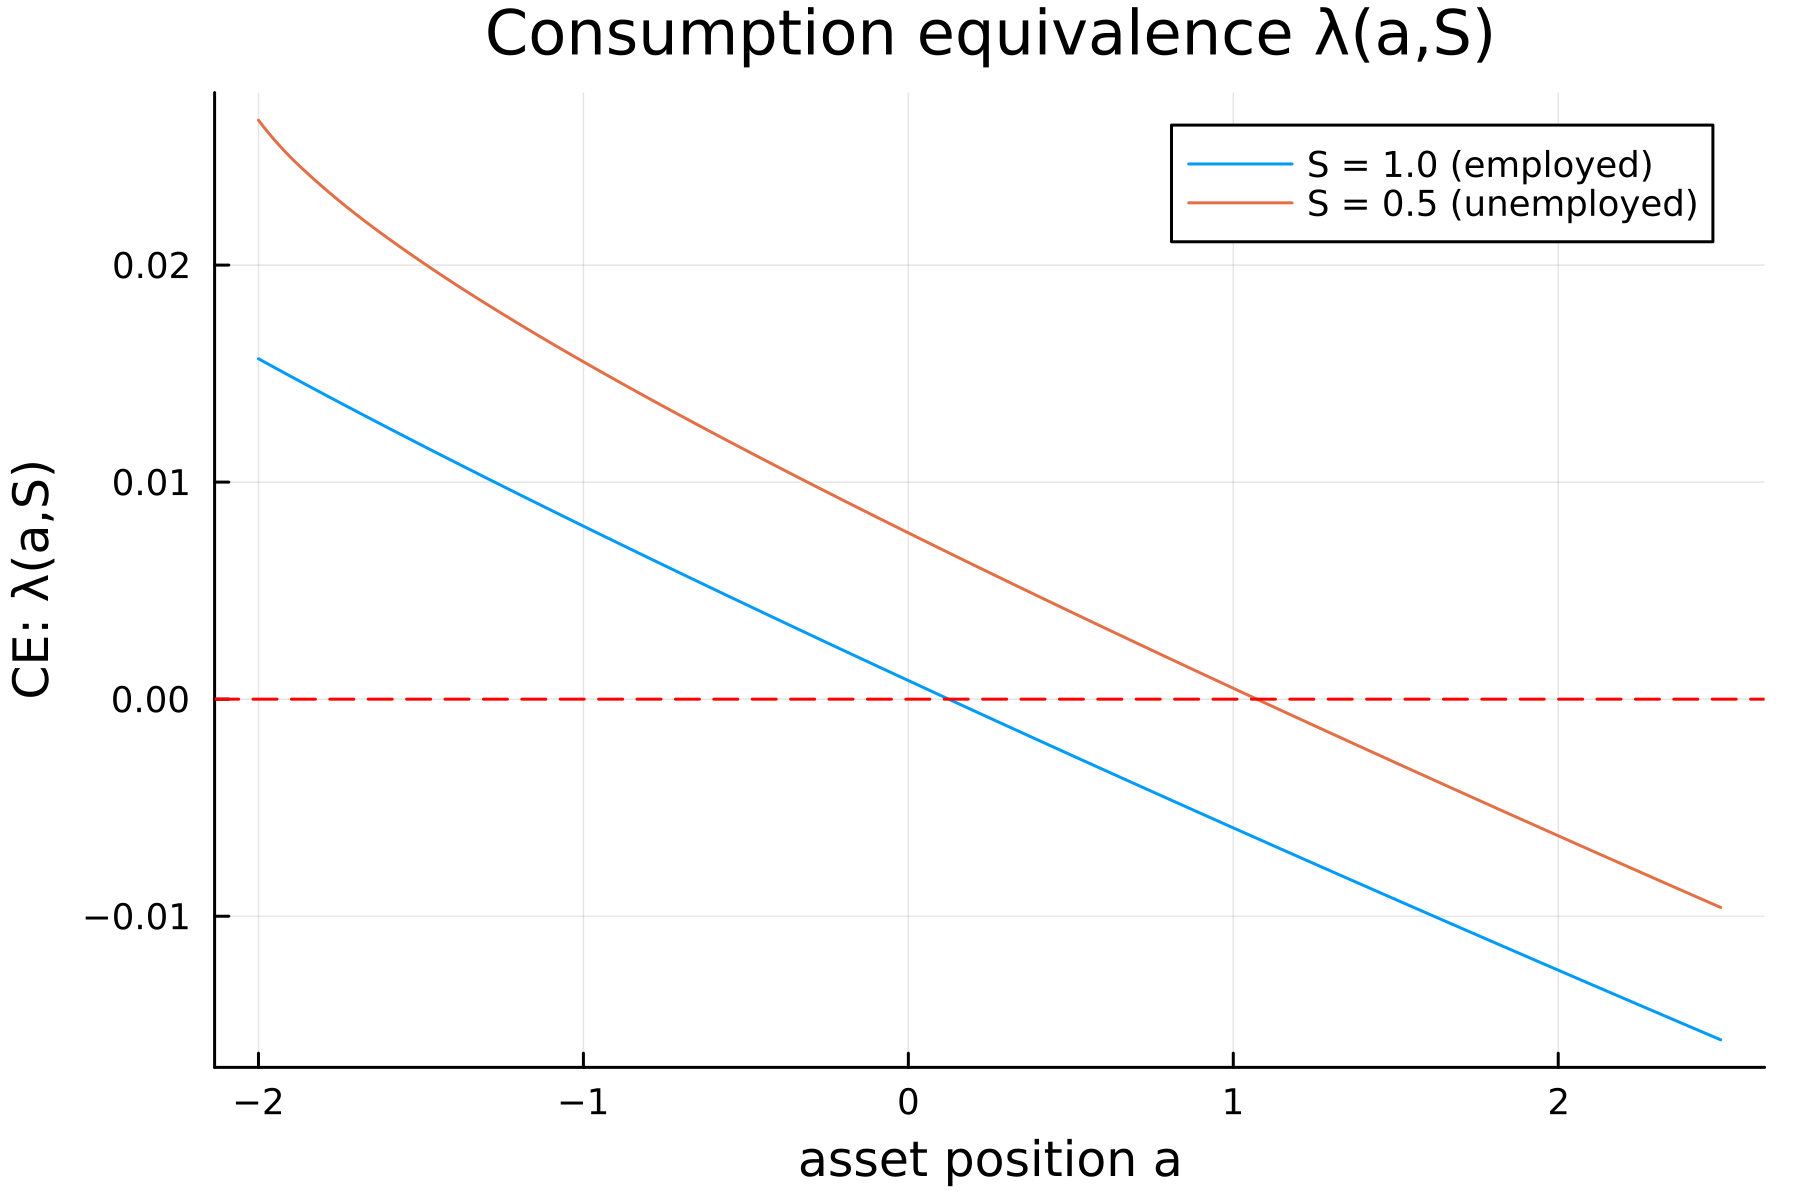
\includegraphics[width=0.6\textwidth, angle=0]
        {5 Consumption_Equivalence.png}
        \caption{Consumption Equivalents by Asset and Employment states}
        \label{fig:CE}
    \end{figure}
\end{solution}

\newpage
%%%%% Exercise 3.2
\begin{framedexercise}[Welfare in two markets and welfare gains/losses] The welfare in complete market (henceforce $W^{FB}$) is:
    \begin{eqnarray}
        W^{FB} & = & \E\left[ \sum_{t=0}^\infty \beta^t
            \frac{(c^{FB})^{1-\alpha}-1}{1-\alpha} \right] \\
        & \xRightarrow[\text{\scriptsize stationary}]{\text{\scriptsize $c^{FB}$}} & \sum_{t=0}^\infty \beta^t
        \frac{(c^{FB})^{1-\alpha}-1}{1-\alpha} = \frac{(c^{FB})^{1-\alpha}-1}{(1-\alpha)(1-\beta)}.
    \end{eqnarray}
    The economywide welfare gain (or loss) from switching back to complete market is  given by
    \begin{eqnarray}
        WG = \sum_{(a,s) \in A \times S} \lambda(a,s)\mu(a,s).
    \end{eqnarray} Then, \begin{itemize}
        \item[\circled{1}] What is $W^{FB}$?
        \item[\circled{2}] What is $W^{INC}$, where
              \begin{eqnarray}
                  W^{INC} = \sum_{(a,s) \in A \times \mathcal{S}} \mu(a,s) v(a,s)
              \end{eqnarray}
        \item[\circled{3}] What is $WG$, the welfare gain (or loss) from switching back to complete markets?
    \end{itemize}
\end{framedexercise}

\begin{solution}
    From my Julia terminal, $W^{FB}$ (rounded to 5 digits) is $-4.25252$.
    $W^{INC}$ (rounded to 5 digits) is $-4.45153$. This aligns to class slides,
    \textit{``Aggregate welfare is higher in the complete markets economy than
        the incomplete markets economy (no surprise)''}.
    The welfare gain of switching to complete markets (rounded to 5 digits) is $0.00134$. \qed
\end{solution}

%%%%%% Exercise 3.3
\begin{framedexercise}[Switching back or not] What fraction of the population would favor changing to complete markets?
    That is, \begin{eqnarray}
        \sum_{(a,s) \in A \times S} \mathbb{1}\{\lambda(a,s) > 0\} \mu(a,s).
    \end{eqnarray}
\end{framedexercise}

\begin{solution}
    From my Julia terminal, the fraction of agents that favor switching
    to complete markets (rounded to 5 digits) is $0.54145$.
    This is highlighted by the $\lambda(a,s) \geq 0$ (i.e., above red dashed line) in Figure \ref{fig:CE}. \qed
\end{solution}


%\newpage

%%%%%%%%%%%%%%%%%%%%%%%%% end %%%%%%%%%%%%%%%%%%%%%%%%%%%%%%

\newpage
%\vspace{-2ex}
\printbibliography



\end{document}
